\section{Plant phenotyping}
The terms phenotype and phenotyping are often interpreted in diverse ways between authors and between studies. In order to avoid any confusion, it is important to define these concepts clearly\footnote{An extensive list of all the needed definitions is available in the glossary in the forepart of this thesis.}.
We can define the phenotype as the set of all types of traits of an organism or one of its subsystems. It is often confused with the phenome which is the physical totality of all traits of an organism or one of its subsystems. The same distinctions can be made between the genome and the genotype, where the genome is the physical totality of all genes of a cell, tissue or organism and the genotype is only a set of those genes, distinguished by specific base sequence, or locus \parencite{mahner1997exactly}. We can then re-express the phenotype of an organism as the expression of the genotype as traits in a given environment $(\mathrm{Phenotype} = \mathrm{Gene} \times \mathrm{Environment})$, since the genotype, the environment, and their interaction influence quantitative traits in a complex and dynamic manner.\\
Therefore, plant phenotyping is defined as the identification of effects on the phenotype (i.e., the plant appearance and performance) as a result of genotype differences (i.e., differences in the genetic code) and the environmental conditions to which a plant has been exposed \parencite{houle_phenomics:_2010,fiorani_future_2013}. In this thesis, we refer to phenotyping more precisely as the set of methodologies and protocols used to measure plant growth, architecture, and composition with a certain accuracy and precision at different scales of organization \parencite{fiorani_future_2013}.\\
Phenotyping is more largely part of phenomics, which is defined as the study of plant growth, performance and composition. Forward phenomics uses phenotyping tools to sieve through the available "genetic pool" of a species (the germplasm) for valuable traits. Reverse phenomics is the detailed dissection of traits to reveal mechanistic understanding and often involves reducing the trait to a biophysical processes and ultimately to genes  \parencite{furbank_phenomics_2011}.\\


Plant phenotyping is an important tool to address and understand plant environment interaction and its translation into application in crop management practices, effects of biostimulants, microbial communities, etc \parencite{pieruschka2019plant}. 
The demographic projections show that cereal grain yields must increase by at least 70\% \parencite{furbank2009c4} or even double \parencite{tilman2011global} before 2050 to meet the predicted
production demands of the global population. Even though extensive breeding has been responsible for tripling cereal yield in the last 50 years \parencite{pingali2012green} and production rates are still increasing yearly, annual increases in yield achieved from traditional breeding programs worldwide are no longer sufficient to meet projected demand for all three major cereal crops: rice \textit{(Oryza sativa)}, maize \textit{(Zea mays)} and wheat \textit{(Triticum aestivum)} \parencite{tester2010breeding}.
 In the actual context of climate change, demand for biofuel feedstocks will also undoubtedly increase over the next decade \parencite{sticklen2007feedstock}, resulting in potential
competition for arable land between food and fuel crops. At
the same time the impacts of climate change on global
temperatures and rainfall patterns are likely to lead to
reductions in yields due to abiotic stress \parencite{tester2010breeding}. Therefore, the genetic improvement of crops is imperative to achieve high intrinsic yields and yield stability under abiotic stress, to further ensure future food security. Continuing advances in
the techniques available to breeders offer the potential to
increase the rate of genetic improvement \parencite{phillips2010mobilizing}, and advances in phenotyping are the key to create and offer new methods that will solve the problems that agriculture is currently facing.\\

However, plant phenomics does not consist of solely associating a genotype to one phenotype in a given condition (e.g., in a controlled
environment), but rather in characterizing the plasticity of the
plant phenome when exposed to a range of environmental conditions \parencite{tardieu_plant_2017}. Therefore phenotyping is often a complex task because the plasticity of phenotypes in plants is enormous and plant phenotypic responses are generally characterized by response curves or reactions to the environment, which for complex traits are inherently continuous and mostly nonlinear \parencite{sultan2003phenotypic}. Indeed, plants are not homeostatic for temperature and water under rapidly changing conditions. For example, plant evapo-transpiration can range from 50\% to 200\% of their own weight \parencite{vadez2014transpiration}, leaf temperature can vary by more than 20$^{\circ}$ in a single day, leading to spectacular changes in plant morphology \parencite{caldeira2014hydraulic}. As a consequence, phenotyping also encompasses the characterization of the environment of the plant, but it has long been difficult to record both biological systems and their environment in the multitude of spatial and temporal dimensions that are necessary to understand
the development of a specific phenotype \parencite{pieruschka2019plant}. Mainly because environmental factors influencing plant growth and development are characterized by different levels of heterogeneity in space and time \parencite{hodge2004plastic}.
Another source of complexity is the fact that plants do not have a central organ that acts as a control unit for the entire organism. The control of functions often relies on feedback loops involving exchanges of information. Such exchanges of information operate at short-term scales at the cell or organ levels, and translate into long-term plant or canopy behaviours through whole-plant mechanisms that are highly non-linear. Hence, plant phenomics requires analyses at spatial scales ranging from single cell to canopy, and temporal scales ranging from minutes (for metabolism and hydraulics) to months (for yield) \parencite{tardieu_plant_2017}. Table \ref{tab:phenotyping_scales} gives a quick overview of the different scales present in phenotyping and their associated methods and mechanisms.

\begin{center}
\begin{table}[!htbp]
\noindent 
\caption{Phenotyping at different scales of organization. Redrawn from \cite{tardieu_plant_2017}}
\resizebox{\textwidth}{!}{
\begin{tabular}{p{3.8cm}C{3.4cm}C{3.4cm}C{3.4cm}}
    \toprule
    Typical phenotyping platforms
    & High-precision platforms (omic, anatomy, organ)
    & Whole-plant, multi-environment platforms (field or controlled) 
    & Field multi-environment networks\\
    \midrule
    Level of plant organization
    & Organ
    & Plant or canopy
    & Canopies in a range of environments\\
    \hline
    Typical methods
    & Omics, 4D organ imaging, fluxes 
    & 4D plant/canopy imaging fluxes, sensors 
    & Yield, sensor network, remote sensing\\
    \hline
    Typical mechanism
    &  Hydraulics, metabolism, signalling 
    & Light interception, water transfer, whole-plant signalling
    & Trade-offs between processes \\
    \hline
    Ratio biology/other processes
    & \multicolumn{3}{Sc}{
        \tikz[baseline=(current bounding box.base)]{
            \path[draw=blue,fill=blue!30,thick]
            (0,0.3) -- (8,0.1) -- (8,-0.1) -- (0,-0.3) -- cycle;}
    } \\
    \hline
    Relevance for yield prediction
    & \multicolumn{3}{Sc}{
        \tikz[baseline=(current bounding box.base)]{
            \path[draw=blue,fill=blue!30,thick]
            (0,0.1) -- (8,0.3) -- (8,-0.3) -- (0,-0.1) -- cycle;}
    } \\
    \hline
    Methods for trans-scale communication
    & \multicolumn{3}{c}{
        \tikz[font=\sffamily\small,
            ultra thick, >=Straight Barb,
            baseline=(current bounding box.base)]{
            \path (2,0.3);
            \draw[-latex] (0,0) -- (4,0)
            node[midway, below]{Gene editing, plant simulation};
            \draw[-latex] (4,-1) -- (0,-1)
            node[midway, below]{GWAS, model-assisted dissection};
        }
    } \\
\bottomrule
\end{tabular}}
\label{tab:phenotyping_scales}
\end{table}
\end{center}

\subsection{Phenotyping bottleneck}



Currently, the rate at which phenotypes are extracted in the field or in the lab is not matching the speed of genotyping \parencite{houle_phenomics:_2010}. While genetic editing techniques and genome mapping technologies are blooming, they depend on a similar improvement in phenotyping, since they are key to analyze plant responses to environmental characterization. This issue is creating a phenotyping bottleneck.\\
In the recent years, there has been a significant advance in the large-scale characterization of plant genomes. This is mainly due to advances in molecular profiling techniques such as marker-assisted selection (MAS) and genomic selection tools for specific alleles \parencite{tester2010breeding,jannink2010genomic}, but also to genome sequencing technologies that allow fast and cheap DNA sequencing \parencite{yano2009genome}. The use of model plants, such as \textit{Arabidopsis thaliana} \parencite{atwell2010genome}, and the introduction of suitable statistical packages and bioinformatics tools has lead to fast and inexpensive genomic information. This fast-paced, high-throughput and low-cost genotyping has paved the way for the developement of large mapping populations
\footnote{A population that is suitable for linkage mapping of genetic markers is known as mapping population. Mapping populations are generated by crossing two or more genetically diverse lines and handling the progeny in a definite fashion. Generally, the parents used for hybridization will be from the same species \parencite{singh2015mapping}.} 
\parencite{mcmullen2009genetic}.\\
However, similar advances in phenotyping are now needed to capitalize on those developments and ensure genetic improvement of crops for future food security \parencite{araus_field_2014}. As said previously, the plasticity of the phenotype according to its environment and the heterogeneity of said environment, make it complex to capture plant phenotype in a dynamic and significant way. While this barrier was previously concerning the platforms and equipment (the hardware), non-invasive methods for plant characterization are now blooming \parencite{li_review_2014}. The new weak spots in the phenotyping chains are now the analysis of imaging data (the software), and the need for a comprehensive approach and good data management \parencite{fiorani_future_2013}.\\
Image analysis is an issue due to the challenges in computer visions and data processing. Plants are are self-changing systems with increasing complexity over times and spatial scales that vary from the subcellular level to the large outdoor field. Therefore, image capturing processes go from automatic cell delineation at the microscopic level, to complete 3-D shape reconstruction at the whole plant level \parencite{minervini2015image}. Moreover, the rapid progress that has been made in the development of a wide array of technologies including novel sensors, image analysis, data mining and modelling, now allow plot-level measurements within seconds. The largest limitation to the implementation of phenotyping platforms is not time anymore, but the management of the huge amount of information generated \parencite{cobb2013next,araus_field_2014}.
Image capturing and processing algorithms must deal with this quantity of complex and diverse raw information, and must also be efficient enough to allow automation and create high-throughput phenotyping platforms (HTPP).\\
\textcite{fiorani_future_2013} also specify that the new innovative technologies need to be integrated in a broader multi-faceted approach, to help relieve the phenotyping bottleneck. The same authors consider a generic process scheme for phenotyping in indoor growth facilities in figure \ref{fig:comprehensive_analysis}. They subdivide the phenotyping process in 3 layers: the experimental design layer, is about having adequate, high-capacity, infrastructures for phenotyping to allow high-throughput; the automated analyses layer, encapsulates the need for standardized and well-defined protocols for data collection and analysis, to allow reproducibility; the last layer emphasizes the need for good software for numerical and statistical analysis and metadata for results interpretation. This scheme also describes the need a good understanding of the parameters driving the evolution of the plant characteristics researchers are measuring. It is clearly valuable to identify a set of parameters before wasting resources by measuring a large number of data points, which could be highly autocorrelated or not indicative of the target performance. 

\begin{figure}[hbtp]
    \centering
    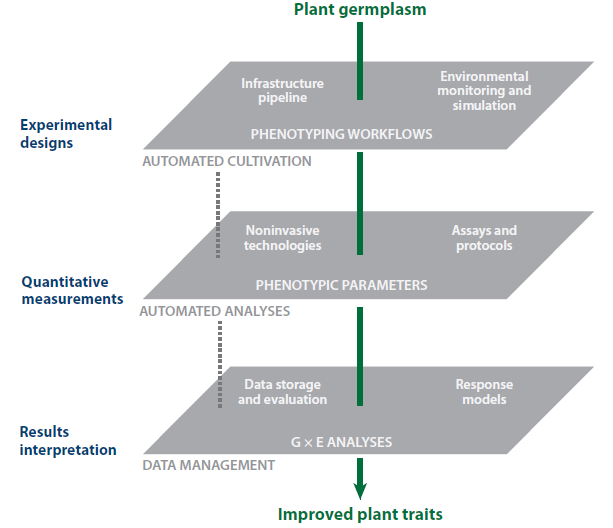
\includegraphics[width=\textwidth]{comprehensive_analysis.PNG}
    \caption[Conceptual scheme for plant phenotyping]{Conceptual scheme for plant phenotyping, applicable in particular to controlled-environment facilities.
Building capacities to screen germplasm for enhanced agricultural traits requires a multidisciplinary
approach. Globally, this scheme offers a quick overview of key layers and elements for a successful implementation of large-scale plant phenotyping. 
%Experimental design includes sufficient capacity to support large-scale phenotyping, including adequate plant growth infrastructure, environmental monitoring and simulation, substrate handling, and, if needed, large-scale biosafety installations. 
%Quantitative analyses strongly benefit from novel noninvasive technologies but require standardized experimental protocols, including sensor calibration and precise definition of raw data processing routines, as part of best practices in phenotyping.
%The data management layer includes hardware for data storage and software for numerical and statistical analyses. Results interpretation requires the integration of experimental metadata within data schemas for the measured phenotypic traits.
This architecture implies a direct link between the measured plant parameters and the environmental conditions, enabling the analysis of gene-environment (G × E) interactions and modeling of phenotypic responses \parencite{fiorani_future_2013}.}
    \label{fig:comprehensive_analysis}
\end{figure}


\subsection{Data processing and standardization in phenotyping}
\subsection{Community integration and collaboration}


\section{Experimental design in field trials}
Experimental field trials in agriculture have always been affected by soil heterogeneity. As \textcite{van_es_1.2_2002} explains, soil is a continuum with variability on multiple scales. 
The heterogeneity is as much affected by microscopic interactions than by field-sized effects. 
Therefore, agricultural trials have always heavily relied on randomisation, blocking and replication to account for spatial variability and remove bias from the estimation of the treatment effects \parencite{atkinson_one_2001}. 
For randomisation to be truly effective, stationarity of the mean and spatial independence assumptions need to be verified. Several studies have proved that it is rare that both these assumptions hold in field trials \parencite{davidoff_method_1986,nielsen_spatial_1973,iqbal_spatial_2005}. 
Moreover, \textcite{van_es_spatial_1993} showed that even randomized designs can still be problematic for experiments with large numbers of treatments and low numbers of replications in the presence of spatial autocorrelation. A new class of design has been proposed involving the use of replicated plots for a percentage of the test lines: the “p-rep” designs \parencite{cullis_design_2006,velazco_modelling_2017}.
Local field trends can influence groups of treatments in specific blocks. As a solution, several authors \parencite{watson_spatial_2000,fagroud_accounting_2002} have suggested considering the spatial trends and autocorrelation structures when creating the design, by using prior soil information, but taking into consideration spatial variability in the design of a trial not only require previous information on the plot but is often costly and cumbersome. 
Furthermore, in practice, most experimenters have neither the capacity to implement advanced designs (in terms of computation power and statistical training), nor the capacity to analyse them. 
Finally, \textcite{van_es_spatially-balanced_2007} showed that completely randomized (43 \% in greenhouse trials) and random block designs (70 \% in field trials) are still vastly used.
Considering this global issue, finding and using an appropriate design is complex task.

\section{Spatial modelling for field trials}

In order to increase the precision of the estimation of genetic effects, experimental designs need to be complemented with appropriate models of analysis. Mixed model analyses using the autoregressive ($AR1$) functions   \parencite{cullis_spatial_1991} have become a standard strategy in field trials. 
However, \textcite{piepho_problems_2015} recently discussed several issues with this model and have therefore proposed the use of the linear variance ($LV$) model \parencite{williams_use_1988} instead. More specifically, \textcite{piepho_linear_2010} have proposed a revised version of this model, augmenting it into two dimensions ($AR1 \times AR1$) The main novelty resides in the addition of spatial components to a classic rows-columns model. Recently, 
\textcite{rodriguez-alvarez_correcting_2018} introduced a novel spatial model that adjusts for both global and local trends simultaneously: the SpATS model (Spatial Analysis of field Trials with Splines). The new spatial method makes use of the  penalized splines \parencite{eilers_flexible_1996} to estimate a bivariate smooth function over the rows and columns of a plot. Using the work of \textcite{lee_efficient_2013,lee_hwang_smoothing_2010,lee_p-spline_2011} the spatial variability is characterized using tensor products of two-dimensional P-splines \parencite{dierckx_curve_1995} and decomposed in a PS-ANOVA system. By exploiting the similarities between P-splines and mixed models \parencite{currie_flexible_2002,durban_adjusting_2001, wand_smoothing_2003}, the P-splines are expressed as a mixed model, which allows the use of classical mixed-model software but also the use of additional random and fixed effects to the model to better capture the variation along the 2-dimensional field.
It has already been tested on simulated data \parencite{rodriguez-alvarez_correcting_2018} and previous field trials data \parencite{lado_increased_2013} and showed promising results.\\

As \textcite{wilkinson1983nearest} highlight, in field trials data modelling, the main components of spatial variation are:
\begin{itemize}
    \item non-stationary large scale (global) variations across the field
    \footnote{\textcite{risser2016nonstationary} defines a stationary process as follows:\\
    Let $C$ be a spatial covariance function, it is said to be stationary if the features of $C$ do not depend on spatial location. More formally, a process $\{Y(\mathbf{s}) : \mathbf{s} \in G\}$ is said to be second-order stationary (or weakly stationary) if the following two properties hold:
    \begin{enumerate}
        \item $E[Y(\mathbf{s})]=E[Y(\mathbf{s}+\mathbf{h})]=c$ for some constant $c$ and 
        \item $C(\mathbf{s}, \mathbf{s}+\mathbf{h})=C(\mathbf{0}, \mathbf{h})$
        for some spatial lag $\mathbf{h} \in \mathcal{R}^{d}$.
    \end{enumerate}
    }
    \item stationary variation within the trial (natural variation or local trend)
    \item extraneous variations (often due to experimental procedures).
\end{itemize}
The spatial variation can also be attributed to systematic effects, e.g. sowing or planting, and random effects such as fertility trends. While systematic effects can easily be modelled using factors and row-columns attributes, it is not case the case for random spatial variation. Since the spatial variation has both random and systematic components, it is straightforward use the mixed model framework.\\
Random spatial variations are harder to model because there are no covariates to relate it to. There are two main approaches to model spatial trends: one based on spatial variance-covariance structures; and the other based on smoothing techniques. Here the yield data, extracted from the phenotyping platform, are modelled using these 2 different models.
\section{Thesis objectives}
This master thesis falls within the scope of the second activity of the European project EPPN2020\footnote{European Plant Phenotyping Network 2020 \url{https://eppn2020.plant-phenotyping.eu/}}. It is a research infrastructure project funded by  Horizon 2020, that will provide access to 31 key plant phenotyping installations. It defines three research activities: (1) novel technologies and methods for environmental and plant measurements, (2) innovative design and analysis of phenotyping experiments across multiple
platforms and (3) a European plant phenotyping information system. The project revolves around data acquisition, data analysis and data networking, so that every platform use common, standardized practices and analysis protocols, that have been verified for robustness and quality.\\

The main goal is to assess the utility of statistical designs and mixed models to identify and correct for spatial trends (heterogeneity) in an aeroponic root installation at UCLouvain (Louvain-la-neuve). The idea is to set up an experiment in this installation using different genotypes (plant varieties) and a custom experimental design to account for possible complex environmental variations. It will be fitted using JMP, taking into account the fact that few replications of the trial will be made and the number of genotype tested. Its efficiency will be tested against classical pre-made designs, such as the Randomized Complete Block (RCB) and alpha-lattice designs, and the best one will be applied on the phenotyping platform. After data collection and image analysis, two different models will be used to model the spatial variability and to assess the quality of spatial prediction. The first one is a two-dimensional version of the linear variance model, revised by \textcite{piepho_linear_2010}. The second one is the SpATS (Spatial Analysis using Tensor product of Splines) model, recently created by \textcite{rodriguez-alvarez_correcting_2018}. These models can be compared using classical precision measures (RMSE,...) but also through more relevant ones like effective dimensions and heritability \parencite{oakey_joint_2006}.\\

The experiment will take place in January in the UCLouvain greenhouses \footnote{A detailed plan of the installation is attached to this document.}. The installation consists of two aeroponic tanks of 495 plants located in a 64 m$^2$ G2 greenhouse. The greenhouse is equipped with temperature and humidity sensors to monitor the local atmosphere. Plants are held on strips, 5 plants per strip, 99 strips per tank. Sprinklers placed at the bottom of the tanks spray nutrient solution on the roots of the 495 plants. Sprinkling solutions and patterns can be customized and even modified during the experiment if needed. Strips move constantly and plants are scanned when the strip passes in front of a camera. This camera consists of a high resolution scanner that captures a full 2D projection of the roots and shoots of each plant. As a full tank revolution takes two hours, plants are imaged every two hours. To ensure minimal manipulation, seed germination occurs within the platform. Experiments usually last 3 weeks, which is the time it takes to the root system to reach a depth of 60 cm. The experiment will include two tanks. In the first one, plants will constantly move to be pictured every 2 hours (usual setup on this platform). In the second one, plants will move twice or three times a day to be pictured. This will allow comparing the effect of moving vs. non-moving plants, which is a feature often available in the phenotyping platforms but poorly evaluated so far.\\

Since the UCLouvain platform focuses on the analysis of the root system, the main variable of interest in the experiment will be the overall growth of the root system of each plant. 
An experiment generates a large amount of data in a raw, image-based format (ca. 200K images). 
Images allow temporal decoupling, provide a condensed set of information and are multi-dimensional (2D usually, but 3D scanning platforms are common \parencite{mooney_developing_2012}). 
A lot of tools are available for data analysis in phenotyping platforms \parencite{lobet_online_2013}. This makes the choice complicated for an external user, especially since most of these software are designed for a single specific purpose. Another challenge in root system architecture (RSA) characterisation is the inherent complexity of the system. Different techniques have been developed to best characterize the RSA in a cost-efficient way \parencite{pound_rootnav:_2013,lobet_novel_2013}. 
Scientists of the UCLouvain platform have developed pipelines\footnote{Here, pipelines are defined as computer programs designed to analyse raw data from phenotyping platforms.} that allow easy processing of the images captured in the platform to extract quantitative root architecture information for the spatial models \parencite{lobet_novel_2013,lobet_novel_2011}.\\

This thesis can be summarised in four main points: create an appropriate experimental design for a phenotyping experiment, analyse data from a high-throughput platform, comparing the efficiency of various spatial models to correct for heterogeneous and non-linear spatial trends and developing the appropriate R scripts.